\title{VerifiQuant: Governance-by-Execution for Financial LLM Workflows}

\author{Anonymous Author(s)}
\affiliation{\institution{Anonymous Institution}\country{}}

\begin{abstract}
Large language models embedded in financial workflows fail most dangerously not by being uncertain, but by being confidently unverifiable.
They emit well-formed numbers without exposing whether the right formula, inputs, assumptions, or boundary conditions were used.
We argue that the central deployment problem is therefore \emph{governability}, not raw accuracy.
A financial reasoning system must know when it is in scope, validate the data it binds, disclose ambiguities before they become hidden assumptions, and refuse in a way that is structured enough to audit.
\textbf{VerifiQuant} implements this view as \emph{governance by execution}.
Each formula family is compiled into a \emph{Financial Inference Contract}.
The contract contains retrieval metadata, typed inputs, deterministic code, invariants, and declared semantic ambiguities.
Each query then passes through a six-layer diagnostic funnel.
Its exits are legitimate outcomes rather than failures of the system.
The LLM is kept at the interface layer. It selects contracts, binds values, and surfaces ambiguities.
Financially consequential computation and repair are deterministic, logged, and cross-verified against contract-declared relations.
Experiments on formula-grounded financial numerical reasoning show that executed controls produce selective abstention, lower silent-wrong risk, and post-hoc failure attribution in ways that prompting the same governance language does not reproduce.
We are explicit about the boundary: a retrieval-grounded execution baseline matches VerifiQuant on well-posed clean questions, so clean-set scalar accuracy is not our claim.
The two separate on governance-perturbed inputs, where executed gates cut false numeric acceptance that the same baseline, prompted with the identical governance taxonomy, does not.
The result is a system that treats an auditable refusal as a first-class financial output, not as a fallback when generation fails.
\end{abstract}
%% OLD ABSTRACT (replaced 2026-07-13, kept for reference)
%% Large language models are increasingly embedded in financial workflows, yet they are governed, if at all, by prompts and post-hoc review.
%% We argue that the central deployment risk is not accuracy but \emph{governability}: a production financial reasoning system must declare its scope boundaries, refuse structurally when it cannot verify its own reasoning, expose audit-replayable decision traces, and numerically cross-verify every repair it applies against a contract-declared algebraic relation at the exact binding being repaired.
%% We present \textbf{VerifiQuant}, a framework that compiles these governance controls into the reasoning pipeline itself, scoped to the \emph{formula-grounded numerical core} of financial workflows: questions whose answer is a deterministic computation over extractable inputs.
%% Each financial formula family is represented as a \emph{Financial Inference Contract} (FIC): retrieval metadata, deterministic executable code, invariants, and declared semantic ambiguities. Every query passes through a six-layer diagnostic funnel in which each layer (M, N, F, E, I, C) is a legitimate, auditable exit.
%% Semantic repairs are restricted to \emph{verifiable atomic transforms} whose numerical effect is cross-checked against a declared algebraic identity before acceptance.
%% On 250 FinanceReasoning questions spanning medium and hard tiers, VerifiQuant reaches \vqAccAll{} accuracy with a silent-wrong rate of \vqSWRAll{}, dominating chain-of-thought baselines on \emph{both} axes at their respective operating points: the strongest CoT+oracle configuration reaches \cotoAccAll{} accuracy with \cotoSWRAll{} SWR, and the gap widens with difficulty (\vqSWRatioMed{} lower SWR on the medium tier, \vqSWRatioHard{} on hard).
%% In fully autonomous operation ($K{=}1$, no clarification) VerifiQuant reaches 81.2\% accuracy with 2.8\% SWR at 84\% coverage; the headline \vqAccAll{} is clarification-assisted recoverability, and under matched coverage the deployed abstention policy exceeds even a perfect-rejector upper bound for the single-shot baseline.
%% Its abstention is selective in a way prompting cannot replicate: on formula families absent from the contract library it abstains 88.9\% of the time versus 19.6\% on covered families, while a refusal-permitted CoT baseline shows almost no such separation.
%% Every residual VerifiQuant failure is post-hoc localized to one of three pre-declared frontier classes: the three pipeline steps where the LLM still acts (selection, binding, hint recall). Mechanizing one of them (declared-hint recall) already cuts overall SWR to 1.2\% and the medium tier to 0\%, at an explicit 1.6-point coverage cost.
%% On contract-grounded adversarial traps the funnel cuts silent-wrong rates from 90\% to 20\% (boundary violations) and 100\% to 10\% (ambiguity).
%% Critically, governance did not transfer through prompts in our experiments: injecting the complete diagnostic taxonomy into oracle prompts \emph{degrades} accuracy under blind review, and prompted refusal misfires on the wrong questions.
%% In our setting, describing governance in prompts did not reproduce the selectivity or attribution of executed controls.
%% END OLD ABSTRACT
%% OLD ABSTRACT (replaced 2026-07-24, kept for reference)
% \begin{abstract}
% Large language models embedded in financial workflows fail most dangerously by emitting \emph{silent wrongs}: confident, well-formatted, wrong numbers carrying no signal that distinguishes them from correct ones. Chain-of-thought baselines do so on \cotSWRAll{} of 250 financial questions, rising on the hard tier.
% We argue the central deployment risk is therefore \emph{governability}, not accuracy: a production system must declare its scope, validate its inputs, disclose its assumptions, and refuse structurally when it cannot verify its own reasoning.
% \textbf{VerifiQuant} compiles these controls into the pipeline itself: each formula family becomes a \emph{Financial Inference Contract} (retrieval metadata, deterministic executable code, invariants, declared semantic ambiguities); every query passes a six-layer diagnostic funnel (M/N/F/E/I/C) whose gates are structured, auditable exits; and repairs are restricted to atomic transforms numerically cross-verified against a contract-declared relation at the exact binding being repaired.
% The LLM selects, binds, and flags. It never computes.
% Operating fully autonomously ($K{=}1$), VerifiQuant answers 84\% of the questions with 81.2\% overall accuracy and a 2.8\% silent-wrong rate, versus \cotSWRAll{} for single-shot CoT and \cotoSWRAll{} for the strongest CoT-plus-oracle baseline; its real risk--coverage operating point exceeds the single-shot baseline's perfect-rejector upper bound at matched coverage.
% With a ground-truth-blind clarification oracle ($K{=}3$), abstentions convert into correct answers and accuracy reaches \vqAccAll{} at \vqSWRAll{} SWR. We report this separately as \emph{recoverability}, not autonomous accuracy.
% A mutation audit of the repair verifier over 179 declared transforms rejects 97.7\% of non-equivalent wrong patches, with structural attacks rejected at 100\%.
% The abstention is selective where prompting is not: the system abstains on 88.9\% of formula families absent from its contract library versus 19.6\% of covered ones, cuts silent-wrong rates on contract-grounded traps from 90\% to 20\% (boundary violations) and 100\% to 10\% (ambiguity), and every residual failure is post-hoc localized to one of three pre-declared LLM-mediated steps. Mechanizing one of them (declared-hint recall) further cuts overall SWR to 1.2\%.
% In our setting, describing governance in prompts did not reproduce the selectivity or attribution of executed controls.
% All claims are scoped to formula-grounded financial numerical reasoning: questions whose answer is a deterministic computation over inputs extractable from the given context.
% \end{abstract}

\begin{CCSXML}
<ccs2012>
<concept><concept_id>10010405.10003550</concept_id><concept_desc>Applied computing~Economics</concept_desc><concept_significance>500</concept_significance></concept>
<concept><concept_id>10010147.10010178</concept_id><concept_desc>Computing methodologies~Artificial intelligence</concept_desc><concept_significance>500</concept_significance></concept>
</ccs2012>
\end{CCSXML}
\ccsdesc[500]{Applied computing~Economics}
\ccsdesc[500]{Computing methodologies~Artificial intelligence}
\keywords{financial reasoning, LLM governance, selective prediction, neuro-symbolic systems, auditability}

\maketitle

%% ===== NOTE [CORE, keep] Introduction: reframe (reliability includes query
%% qualification) + 3 failure modes + contributions. Contribution 2 = the balance
%% thesis (clean parity + malformed-input safety; OOD is a disclosed trade-off). =====
\section{Introduction}
Financial institutions are deploying large language models (LLMs) in workflows that end in numbers: valuation memos, portfolio analytics, client-facing calculators, regulatory reports.
Benchmark accuracy on financial question answering has climbed steadily.
It is tempting to treat the remaining gap as an accuracy problem, one more model generation away from solved.
We argue this framing misses what actually blocks deployment.
A financial LLM workflow fails in production not primarily because it computes the wrong number, but because \emph{nobody can govern how it computes any number}.
Three failure modes, all invisible to headline accuracy, illustrate the gap.

\emph{Silent wrongs.}
The model outputs a confident, well-formatted, wrong number, with no signal distinguishing it from a correct one.
In our experiments a chain-of-thought (CoT) baseline produces confident unflagged wrong answers on \cotSWRAll{} of 250 financial questions.
The rate rises to \cotSWRHard{} on the hard tier.
On adversarially perturbed inputs, it reaches up to 100\% for some perturbation classes (\S\ref{sec:trap}).

\emph{Audit gaps.}
When a loss occurs, the institution must reconstruct \emph{which} formula was applied, \emph{which} inputs were bound, and \emph{why} the system did not stop.
CoT traces cannot serve this role.
They are sampled and non-reproducible.
As the faithfulness literature shows, they are also not causally connected to the computation that produced the answer \cite{turpin2023language,lanham2023measuring}.
Notably, this disconnect \emph{worsens} with model capability, so waiting for stronger models does not close the audit gap.

\emph{Boundary failures.}
Asked a question outside its competence, such as an exotic derivative it has no procedure for, the system answers anyway.
It often silently substitutes a different question it \emph{can} answer.
In our trap study, for example, a baseline responds to a ``Heston stochastic volatility'' request by computing an unrelated manufacturing ratio from the surrounding context.

Regulatory frameworks for high-risk AI converge on a common demand.
This includes model-risk guidance \cite{fed2011sr117}, the EU AI Act's logging provisions \cite{euaiact2024}, and FINRA's supervisory-control expectations \cite{finra2020ai}.
Systems must declare their boundaries, log reproducibly, expose checkpoints for human intervention, and constrain internal modification (\S\ref{sec:governance}).
Today these demands are met, when at all, by \emph{prompt instructions} and \emph{post-hoc review}: governance described in natural language and hoped for at runtime.

\textbf{Our position is that governance controls must be executed, not merely described.}
VerifiQuant operationalizes this position through three mechanisms:

\begin{enumerate}
    \item \emph{Financial Inference Contracts (FICs).}
    Each formula family is compiled offline into a machine-readable contract containing retrieval metadata, typed inputs, deterministic executable Python, numerical invariants, scale checks, and \emph{declared semantic ambiguities}, such as period timing, percent-versus-decimal conventions, and unit bases.
    The LLM never performs arithmetic; it only selects contracts, binds fields, and identifies ambiguities within contract-declared bounds.

    \item \emph{A six-layer diagnostic funnel (M/N/F/E/I/C).}
    Every query passes through gates for intent (M), scope (N), schema completeness (F), boundary validity (E), semantic ambiguity (I, divided into blocking I\textsubscript{HARD} and warning I\textsubscript{SOFT}), and deterministic computation (C).
    Each gate supports a legitimate, structured exit with machine-readable diagnostics rather than a prose apology.

    \item \emph{Verifiable atomic transforms.}
    When clarification changes the required computation, repairs are restricted to bounded transforms.
    A transform is accepted only when its numerical effect satisfies a declared algebraic identity under cross-verification.
\end{enumerate}

\textbf{Contributions.}

\begin{enumerate}
    \item \emph{Architecture.}
    We reframe financial LLM reliability to include \emph{query qualification}---whether a question is in scope, complete, bounded, and unambiguous---not merely answer correctness, and compile six regulator-demanded controls (Table~\ref{tab:spine}) into an executable pipeline.
    The pipeline combines Financial Inference Contracts, the M/N/F/E/I/C diagnostic funnel, and cross-verified atomic transforms (\S\ref{sec:method}).
    Refusal, clarification, and repair become first-class, auditable outcomes.

    \item \emph{Clean accuracy \emph{and} malformed-input safety---not peak accuracy.}
    On 250 FinanceReasoning \cite{tang2025financereasoning} questions (180 medium, 70 hard), a strong \emph{retrieval-grounded execution} baseline (R-PAL: the same top-4 contract retrieval feeding a program the model writes and we execute deterministically) \emph{matches} VerifiQuant on clean, well-posed questions (\rpalAccAll{}/\rpalSWRAll{} SWR vs \vqAccAll{}/\vqSWRAll{}, statistically indistinguishable; single-shot CoT trails at \cotAccAll{}/\cotSWRAll{}).
    Clean-set scalar accuracy is therefore \emph{not} our claim.
    The advantage appears on \emph{malformed} inputs that have no valid answer: on contract-derived governance perturbations VerifiQuant's false numeric acceptance is \govVQfnar{}, against \govPlainFnar{} for plain R-PAL and \govPromptFnar{} for the \emph{same} R-PAL prompted with the full governance taxonomy (\S\ref{sec:trap})---here a confident number is by construction wrong, and executed gates intercept where execution and prompting force-fit.
    No competitor holds both ends: CoT lacks the clean accuracy, R-PAL lacks the malformed-input safety.
    Out of library we report an honest \emph{trade-off}, not a third win: R-PAL answers more out-of-library questions correctly (\oodRPALcorrOOD{}) than VerifiQuant, which abstains selectively; VerifiQuant trades coverage for a scope signal---a verified/unverified boundary---whose value is conditional on needing provenance, and it does \emph{not} lower silent-wrong risk out of library (\S\ref{sec:oodfam}).
    The safety advantage is architectural: neither prompted taxonomy nor refusal-permitted prompting reproduces it.

    \item \emph{Recoverability.}
    We distinguish autonomous operation ($K{=}1$: 81.2\% accuracy, 2.8\% SWR) from clarification-assisted recovery ($K{=}3$: \vqAccAll{} accuracy).
    We position both settings on a risk--coverage curve against a perfect-rejector bound.
    We further localize every residual failure to one of three LLM-mediated steps and disclose the oracle's intent-specification strength as an upper-bound-style caveat (\S\ref{sec:kablation},~\S\ref{sec:attribution}).
\end{enumerate}


\emph{Scope of claims.}
This paper's evaluated territory is the formula-grounded numerical core: single questions whose answer is a deterministic computation over inputs extractable from the given context.
Production financial workflows add multi-document extraction, tabular and PDF ingestion, conflicting sources, data freshness, jurisdiction-dependent accounting policy, and non-numerical judgment.
Our deployed demonstration system already ingests PDF and tabular context, but none of the claims here depend on it.
``Governance-by-execution'' is evaluated for the reasoning core, not the full document-to-decision pipeline.

%% ===== NOTE [CORE, keep] Governance Problem: Table 1 (C1-C6 -> mechanism -> evidence)
%% is the spine. 2.1/2.2 prose compressible for 8pp; keep the spine table. =====
\section{The Governance Problem}\label{sec:governance}

\subsection{What deployment actually requires}
Model-risk guidance (SR~11-7) requires that a model \emph{identify its own failure regimes} and enforce output boundaries rather than extrapolate \cite{fed2011sr117}.
The EU AI Act (Art.~12--13) requires event logging sufficient to \emph{trace any output back to its inputs}, reproducibly \cite{euaiact2024}.
FINRA supervisory guidance requires \emph{explicit human checkpoints} where the system cannot autonomously resolve ambiguity, and that internal modifications be bounded and reviewable \cite{finra2020ai}.
Table~\ref{tab:spine} restates these demands as six concrete controls.
Each control is paired with the mechanism that executes it and the experiment that tests it.
\S\ref{sec:method} walks the mechanism column.
\S\ref{sec:results}--\ref{sec:analysis} walk the evidence column.

\begin{table}[t]
\caption{Governance controls $\rightarrow$ executing mechanism $\rightarrow$ evidence.}
\label{tab:spine}
\small
\begin{tabular}{@{}p{0.16\linewidth}p{0.30\linewidth}p{0.40\linewidth}@{}}
\toprule
Control & Mechanism (\S\ref{sec:method}) & Evidence \\
\midrule
C1 boundary declaration & M/N structured refusal & OOD abstain \oodRPALabsOOD{}$\rightarrow$\oodVQabsOOD{} (selective; \S\ref{sec:oodfam}); M qualitative; MAS baseline $\rightarrow$ 14\% SWR \\
C2 input validation & deterministic E-checks & trap-E: FNAR 90\%$\rightarrow$10\% \\
C3 ambiguity disclosure & I\textsubscript{HARD} block / I\textsubscript{SOFT} warning & trap-I: FNAR 95\%$\rightarrow$20\% \\
C4 cross-verified repair & atomic transforms (AST bounds + point-of-use numeric check) & worked example \S\ref{sec:transforms} \\
C5 audit-replayable trace & DiagnosticReport + deterministic execution & bit-replay from stored bindings; 4 reruns: outcome variance $=0$ \\
C6 abstention as control & selective-prediction exits at every gate & residual-failure attribution \S\ref{sec:attribution} \\
\bottomrule
\end{tabular}
\end{table}

\subsection{Why existing approaches do not provide these controls}
\emph{Execution-based reasoning} (PAL \cite{gao2023pal}, Program-of-Thoughts \cite{chen2023pot}) delegates arithmetic to an interpreter and addresses C-class errors.
But a syntactically perfect program can still encode the wrong financial semantics.
For example, it may compute an end-of-period annuity when the question implies beginning-of-period.
The interpreter neither detects this error nor produces structured attribution.
\emph{Neuro-symbolic translation} (Logic-LM \cite{pan2023logiclm}, LINC \cite{olausson2023linc}, SATLM \cite{ye2023satlm}) obtains formal guarantees by translating natural language into solver input.
But the translation step is the dominant error source.
Recent analysis also argues that specification synthesis is undecidable in general \cite{zhou2026formaljudge}.
VerifiQuant moves the formalization burden \emph{offline}.
Contracts are built and validated at build time, so runtime only selects and binds within a pre-verified space.
\emph{Multi-agent and self-reflection systems} rely on natural-language consensus between agents.
Failures propagate silently across agent boundaries \cite{cemri2025mas}.
We reimplement a nine-node financial multi-agent system \cite{kundu2025multiagent}.
Even with oracle support, it never triggers its own \texttt{ask\_human} node and delivers 14\% SWR on the canonical 50-question subset.
It has a human-checkpoint \emph{node}, but no executed \emph{control} that routes to it.
\emph{Prompted refusal} is the cheapest candidate control.
\S\ref{sec:analysis} shows that it is non-selective.

%% ===== NOTE [METHOD/CORE] Method: FIC + M/N/F/E/I/C funnel + verifiable transforms.
%% 3.4 transforms + RepairBench (Table 3) = C4 supporting mechanism; compressible for 8pp
%% (RepairBench table could move to ACL). Funnel (3.2) and OITL (3.3) are load-bearing. =====
\section{Method}\label{sec:method}

\subsection{Financial Inference Contracts}
An FIC packages one formula family as three artifacts keyed by \texttt{fic\_id}.
The \emph{retrieval card} carries selection hints, applicability and non-applicability conditions, scope boundaries, and keywords, used by BM25 plus an LLM selector to decide whether the contract applies.
The \emph{core card} carries typed inputs, deterministic \texttt{compute} code in plain Python, numerical invariants and scale checks (E-checks), and \texttt{semantic\_hints} for known ambiguities.
Each hint declares resolution options, a default, and a hard/soft level.
The \emph{repair card} maps each diagnostic outcome to one of eight structured actions (request missing fields, present clarification options, declare scope boundary, \ldots), each declaring its legal next-step transitions.
The LLM's role is \emph{mapping into contracts}: selecting, binding, and flagging.
It never performs the financial computation.
Contracts are themselves governed at build time.
E-check expressions are lint-gated against the exact evaluation namespace used at runtime.
Every card passes execution smoke tests, and a pre-declared output-type policy is enforced by audit.
\S\ref{sec:attribution} shows this audit catching real defects.

\subsection{The M/N/F/E/I/C diagnostic funnel}
Given a question and context, gates fire in order:
\textbf{M} (intent): does the question map to exactly one contract family? Exit: structured disambiguation request.
\textbf{N} (scope): is any contract applicable? Exit: scope-boundary refusal.
\textbf{F} (schema): are all required inputs present? Exit: slot-filling request with \texttt{requested\_fields}.
\textbf{E} (boundary): do bound inputs satisfy invariants and scale checks? Exit: deterministic alert naming the violated check.
\textbf{I} (ambiguity): does an unresolved declared ambiguity change the computation (I\textsubscript{HARD}: block and clarify) or only its interpretation (I\textsubscript{SOFT}: proceed with explicit warning)?
\textbf{C}: deterministic execution with audit log.
Every case yields a $\mathrm{DiagnosticReport}=(\textit{exit\_layer},\textit{fic\_id},\textit{binding},\textit{invariant\_trace},\textit{action})$.
The report is layer-attributable, machine-readable, and \emph{audit-replayable} in a precise sense.
Deterministic execution and invariant evaluation replay exactly from the stored binding.
LLM-mediated selection and binding decisions are logged, so a historical decision can be re-executed as recorded.
Fresh reruns from raw text are \emph{not} guaranteed to take identical paths.
In four independent reruns of the canonical subset, outcomes remain stable while the recovery paths vary.
Abstention is not a fallback; it is the designed output of five of the seven gates (C6).
Figure~\ref{fig:pipeline} annotates each gate with the control it executes.

\begin{figure*}[t]
\centering
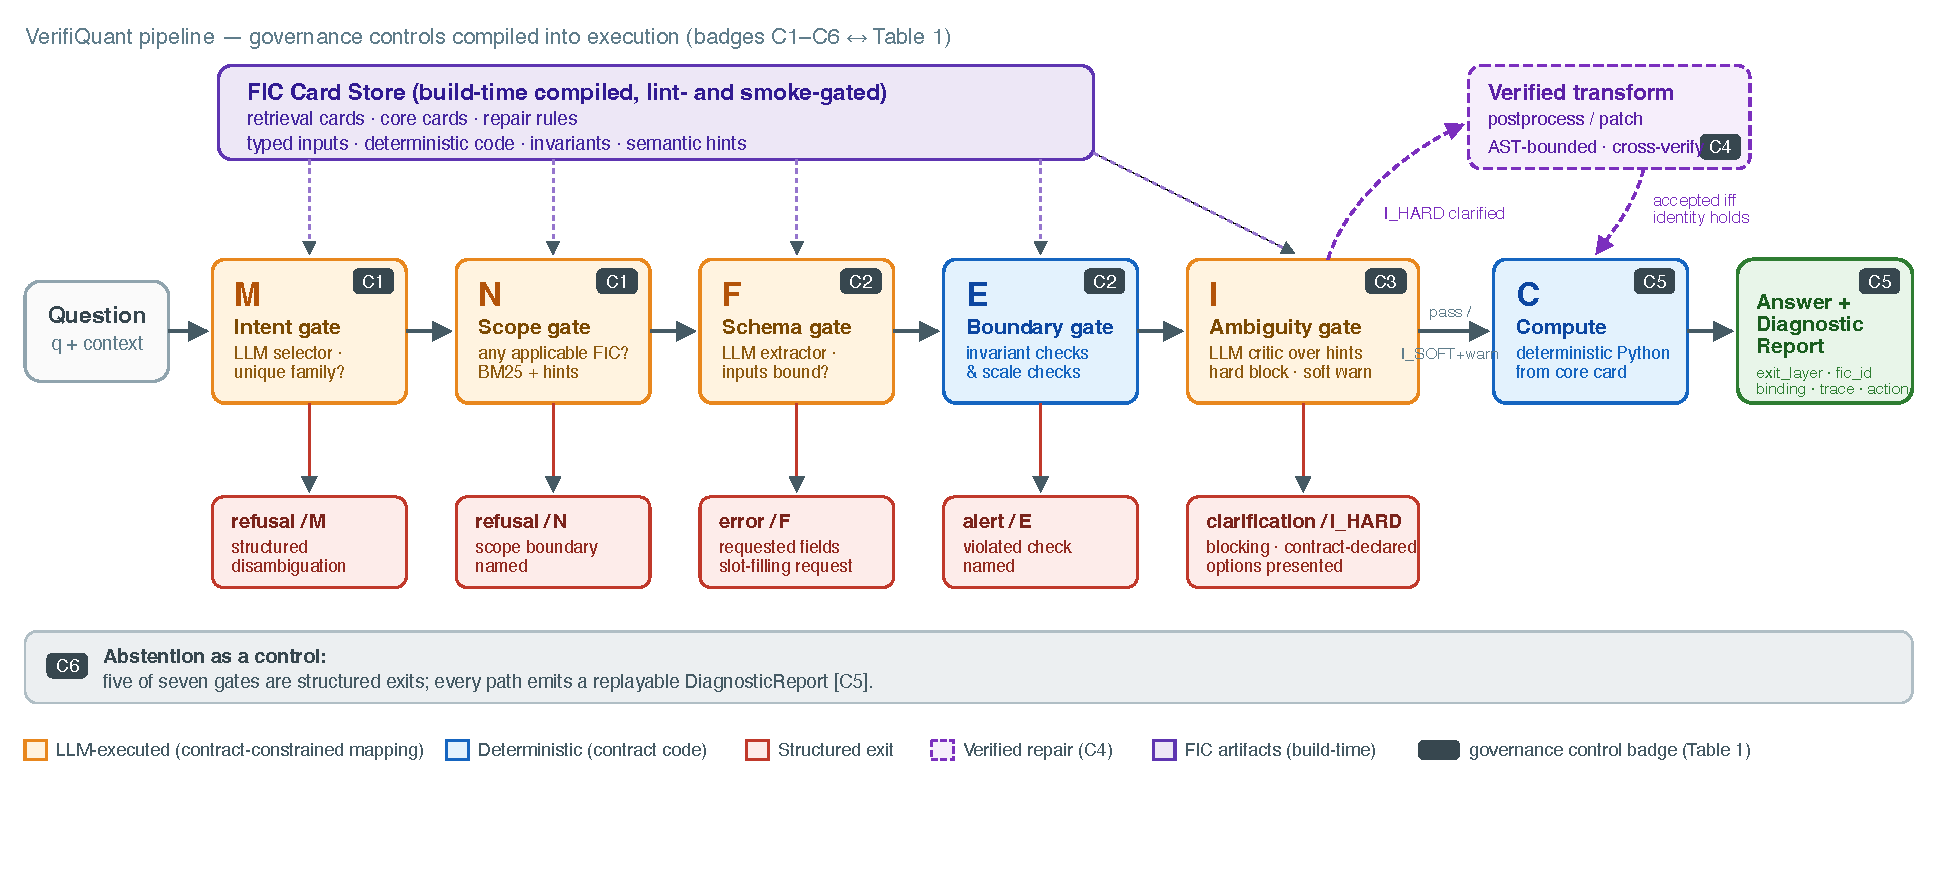
\includegraphics[width=0.9\linewidth]{figures/fig1_pipeline.pdf}
\caption{The VerifiQuant pipeline.
LLM components (orange) only map into contracts; all financially consequential computation is deterministic (blue).
Five of seven gates are structured exits (red); repairs go through verified atomic transforms (purple).
Badges C1--C6 reference Table~\ref{tab:spine}.}
\label{fig:pipeline}
\end{figure*}

\subsection{Oracle-in-the-loop evaluation protocol}\label{sec:oitl}
To measure \emph{recoverability}, we ask how far the framework gets when intent is clear but the answer is unknown.
A constrained oracle agent simulates an ideal clarifying user.
Per turn the oracle reads the current DiagnosticReport and the question's ground-truth \emph{computation code} (the intent specification) but never the numeric answer; it may only rewrite question/context, never inject values.
Iteration is capped at $K{=}3$.
The same GT-blind discipline applies to all CoT+oracle baselines.
The oracle reviews every turn (blind review), receives no correctness signal, and never sees the numeric ground truth.
Otherwise, ``intervene only when wrong'' would itself leak the label.
Across all oracle configurations $\mathrm{broken\_count}=0$: blind review never corrupted a correct answer.

\subsection{Verifiable atomic transforms}\label{sec:transforms}
When an I\textsubscript{HARD} clarification changes the required computation, free-form code regeneration would reopen the door the funnel just closed.
VerifiQuant permits exactly two repair forms.
\emph{result\_postprocess}: a pure-arithmetic expression over the original result and bound inputs (e.g., $r \times (1+i)$), bounded by an AST node-count limit, a safe-name whitelist, and a numerical invariant check.
\emph{code\_patch}: a single-site textual replacement in contract code (e.g., \texttt{start=1} $\rightarrow$ \texttt{start=0}).
It is accepted only if the pattern occurs exactly once, the shallow AST diff stays within a declared blast radius, and no new imports or dangerous calls appear.
The decisive check is \emph{cross-verification}: the patched code's output must equal the declared algebraic identity applied to the original output on multiple sampled inputs.
\emph{Worked example (annuity timing).} A contract computes an end-of-period annuity (579.98).
The user clarifies that payments occur at period start.
The system applies the pre-declared post-process \emph{and} the code patch, then reruns both.
Both yield 577.10, so the repair is accepted and logged with its invariant.
A code change is admissible only when its numerical effect is cross-checked against the declared relation.
The check does not trust the LLM that proposed the change (C4).
\emph{Scope of the guarantee.} This is bounded repair validation, not formal equivalence.
The check is numerical, applied at the point of use, and conditional on the contract-declared invariant.
A repair is deployed on one binding, and the invariant is verified at that binding.
The invariant is a static, reviewable, versioned build-time artifact rather than runtime LLM output.
Two coincident errors would still pass: a wrong invariant and a patch wrong in exactly the compensating way.
Single-sided errors are caught.
We deliberately avoid claiming formal verification.
Earlier symbolic-proof prototypes were too brittle for this heterogeneous formula library, so the paper claims bounded numerical validation instead.

\emph{RepairBench: what the verifier actually catches.}
Beyond the worked example, we mutation-test the verifier over every synthesizable \texttt{result\_postprocess} spec in the 250-card library.
This covers 179 specs across 149 formula families.
Each spec is paired with six programmatic wrong-patch classes proposed against the \emph{unchanged} contract invariant (Table~\ref{tab:repairbench}).
Structural attacks (function-call injection, AST-bound breach) are rejected at 100\% by the static guards.
Of 879 non-equivalent semantic mutants (27 arithmetically-equivalent mutants excluded), \textbf{97.7\%} are rejected.
Most are rejected by the numerical invariant check.
The 20 residual false accepts are conditional transforms whose guard branch the sampled inputs did not exercise.
Legitimate declared transforms pass at 96.1\% (172/179).
The 7 rejections are contract defects where the declared invariant and expression disagree.
Thus, the checker also audits the contracts themselves.
This 97.7\% is a rejection rate under our six-operator mutation distribution.
It is not an estimate that a real LLM-generated wrong repair is caught.

\begin{table}[t]
\caption{RepairBench: mutation testing of the transform verifier (C4) over 179 transform specs / 149 families, zero LLM calls.
Each mutant is proposed against the unchanged contract invariant.
``True FA'' $=$ false accepts after excluding arithmetically equivalent mutants; the effective total is over non-equivalent mutants.}
\label{tab:repairbench}
\small
\begin{tabular}{@{}lrrr@{}}
\toprule
Mutation class & $n$ & Rejected & True FA \\
\midrule
function-call injection & 179 & 100\% & 0 \\
oversized AST & 179 & 100\% & 0 \\
operator swap & 171 & 93.0\% & 4 \\
coefficient perturbation & 164 & 92.7\% & 3 \\
variable swap & 34 & 85.3\% & 3 \\
identity (no-op) & 179 & 89.9\% & 10 \\
\midrule
non-equivalent total & 879 & \textbf{97.7\%} & 20 (2.3\%) \\
\bottomrule
\end{tabular}
\end{table}

%% ===== NOTE [CORE, keep] Protocol: datasets (in-library disclosure + contamination
%% control + cost) and baselines (CoT / plain PAL / R-PAL / R-PAL+ / VQ). The in-library
%% disclosure is load-bearing honesty; keep. =====
\section{Experimental Protocol}\label{sec:protocol}

\subsection{Datasets}
\textbf{Clean set (main).} 250 questions from FinanceReasoning \cite{tang2025financereasoning}: 180 medium (difficulty 2.48--4.14) and 70 hard (4.16--7.19), stratified by difficulty quartile at seed 42; question IDs are committed.
FinanceReasoning is a re-annotated union of four public financial sub-corpora (CodeFinQA, CodeTAT-QA, FinCode, FinanceMath) plus expert-verified problems built from an Investopedia-derived function library.
We draw our 250 questions from that last, function-linked subset.
Each selected question carries a reference-function identifier, and that linkage is what makes a contract library constructible; the four re-annotated sub-corpora lack it.
To our knowledge FinanceReasoning is the only financial-reasoning benchmark that ships a per-question link to a formula-level reference implementation, so we treat the link as a prerequisite, not a design variable: the alternative---hand-annotating formulas onto answer-only corpora---would reintroduce the single-annotator bias and answer-leakage our protocol controls.
The consequence is explicit and stated once: our evaluation is \emph{in-library} by construction, not a claim of open-world coverage (\S\ref{sec:oodfam} probes absent-family behavior separately).
The benchmark enforces a strict 0.2\% numerical-error margin, so ``correct'' is demanding, and the hard tier probes governance under difficulty shift.
A canonical 50-question medium subset supports deep protocol validation (oracle grid, ablations, rerun-variance) before the 250Q run.
\emph{Contamination control.}
Each question carries two artifacts: a formula-level \emph{reference function} the family was built from, and a per-question \emph{worked solution} with numbers substituted.
An early pipeline built cards from the worked solutions, compiling each answer into the knowledge base; the final protocol builds cards \emph{only} from the reference functions (FinanceReasoning's separately released 3{,}133 Python routines distilled from 6{,}138 Investopedia articles), never reads the worked solution or gold answer, and deduplicates formula kernels by AST hashing.
We do \emph{not} claim the reference functions are independent of the questions---they generated them---so a card contains, by construction, the formula its question needs; the LLM's task is to route, bind, and gate, never to derive the formula.
Keeping the worked solution out of card construction is what keeps the numeric answer out of the knowledge base.
\emph{Contract engineering cost.}
The 250-card library was generated \emph{fully automatically}: three staged LLM calls per family (core, retrieval, repair) plus deterministic normalization, with the gate battery as quality control.
The build-time record is concrete: execution smoke 0/250 failures; E-check lint auto-repaired 4 expressions on 2 cards; the post-run type audit auto-repaired 4 cards under the pre-declared output policy and surfaced 5 candidates (2 deliberately-array cards confirmed, 3 false positives cleared); all repairs logged, none consulting gold answers.
The cost shifted rather than vanished: the 50Q pilot needed hand repair on 5/50 cards from execution signals alone, whereas at 250 cards automated audits catch and repair the same signal classes and human attention narrows to the flagged candidates.
What survives the gates is \emph{semantic} specification error---the class-B/C/D frontier of \S\ref{sec:attribution}, first mechanically reduced by the hint-trigger pre-pass (\S\ref{sec:recall}).
The honest trade is runtime hallucination for build-time specification error, which is static, per-family localized, and partially auditable without gold answers; we do not measure inter-author consistency (single LLM author) or cross-domain migration cost.

\textbf{Trap set (contract-grounded).} Trap labels guessed from question text are themselves unreliable.
Each trap is therefore derived from a clean question plus its FIC by a deterministic operator.
The label \emph{is} the operator.
\textbf{F} removes a required input.
\textbf{E} injects a boundary-violating value anchored to a declared E-check predicate.
\textbf{I} deletes the disambiguating phrase that re-opens a declared semantic hint, with hard/soft status set by the contract.
\textbf{N} swaps in an out-of-scope ask while keeping the original context.
\textbf{M} replaces the question with under-specified intent.
50 traps (10 per operator), zero \texttt{needs\_review}, manually spot-checked; the M operator retains metric-bearing context and does not isolate a valid trap, leaving 40 evaluable traps (\S\ref{sec:trap}).
%% [ICAIF-CUT: operator examples]
Concretely, an E-trap sets total revenue to $-\$1.2$M, which is financially absurd but syntactically legal.
An I-trap deletes ``expressed as a percentage'', re-opening a declared decimal/percent hint.
An N-trap asks for Heston stochastic-volatility pricing over an untouched manufacturing context.
%% [/ICAIF-CUT]
\emph{Honest scoping:} N is defined relative to the contract library.
For VerifiQuant this is a principled OOD check; for CoT it is an incidental mismatch cue.
The Tier-1 M operator retains metric-bearing context, so it yields no evaluable trap and is excluded from quantitative claims (\S\ref{sec:trap}).

\subsection{Baselines and metrics}
On 250Q, we evaluate CoT single-shot (Gemini 2.5 Flash and Pro), CoT + GT-blind oracle ($K{=}3$, blind review), two execution baselines, self-consistency@5, and VerifiQuant ($K{=}3$, Flash).
In the execution baselines the model writes Python and the code is executed deterministically: \emph{plain PAL} sees no retrieval, while \emph{R-PAL} receives VerifiQuant's identical top-4 contract retrieval as candidate context.
On the contract-grounded trap set we additionally run R-PAL and a taxonomy-prompted variant (R-PAL$^{+}$) as governance controls; each is run three times and scored with the same VerifiQuant scorer, and VerifiQuant is evaluated funnel-only at $K{=}1$.
Self-consistency@5 serves as a realizable confidence proxy (\S\ref{sec:kablation}).
On the canonical 50Q: additionally CoT single-shot/oracle with Gemini 2.5 Pro, plain and funnel-guided oracle prompts, a J.P.\ Morgan multi-agent reimplementation \cite{kundu2025multiagent}, and VerifiQuant Pro.
Following selective prediction \cite{elyaniv2010foundations,geifman2017selective}, every case is \emph{Correct}, \emph{Silent Wrong}, or \emph{Abstention}.
\emph{Silent Wrong} means a confident unflagged wrong number.
Informal no-answers, such as a model declining in prose without diagnostics, are counted as abstention rather than silent wrong for \emph{all} systems.
We report coverage, selective accuracy $=$ Correct/(Correct$+$SW), and \textbf{SWR} $=$ SW$/N$.
SWR is the key deployment-risk metric.
On traps, where no legitimate numeric answer exists, correct behavior is interception; we report trap SWR and the structured-catch rate.

%% ===== NOTE [CORE] Results: opens with the lens frame. Advantage = clean parity
%% (5.1) + malformed-input safety (5.4, main win). OOD (6.1/6.2) is a disclosed
%% trade-off, NOT a win. risk-coverage (5.2) is an ACL-candidate. =====
\section{Results}\label{sec:results}
The organizing question is not which system is most accurate, but which stays reliable across the inputs a deployed workflow actually meets.
Three lenses carry the claim, and a fourth is an honest trade-off.
On \textbf{clean, well-posed} questions execution suffices and R-PAL ties VerifiQuant (\S\ref{sec:main}).
On \textbf{malformed} inputs with no valid answer---missing fields, boundary violations, unresolved conventions---executed gates intercept where execution and prompting force-fit (\S\ref{sec:trap}).
The governance-doesn't-transfer analysis shows the interception is \emph{executed}, not prompted (\S\ref{sec:analysis}).
VerifiQuant is the only system strong at \emph{both} ends: CoT lacks the clean accuracy, R-PAL lacks the malformed-input safety.
The fourth lens, \textbf{out-of-library} coverage (\S\ref{sec:oodfam}), is a disclosed trade-off rather than a win: the baselines stay accurate from parametric knowledge, while VerifiQuant abstains selectively and buys a scope signal at a coverage cost, without lowering silent-wrong risk there.

\subsection{The clean lens: 250 questions, two difficulty tiers}\label{sec:main}
On clean questions the honest finding is a tie at the top.
A retrieval-grounded execution baseline (R-PAL) matches VerifiQuant (\rpalAccAll{}/\rpalSWRAll{} vs \vqAccAll{}/\vqSWRAll{}; accuracy/SWR McNemar $p{=}0.13/0.79$), and both clear the prompt-only baselines: VerifiQuant still dominates \emph{both} CoT configurations on both axes (\vqAccAll{} vs \cotoAccAll{}; \vqSWRAll{} vs \cotoSWRAll{}), a comparison that survives coverage matching (\S\ref{sec:kablation}).
Parity with R-PAL is the boundary of the clean-set claim; the systems separate only under the governance, scope, and coverage lenses that follow, and on attribution.
The oracle helps CoT (77.6\%$\rightarrow$82.0\%) but does not change its failure mode: coverage stays effectively forced, and roughly one answer in seven is a confident unflagged wrong number.
The oracle helps CoT (77.6\%$\rightarrow$82.0\%) but does not change its failure mode: coverage stays effectively forced, and roughly one answer in seven is a confident unflagged wrong number.
\emph{A stronger model does not close the audit gap.} Running the single-shot baseline on Gemini 2.5 Pro lifts accuracy to 82.4\%, matching VerifiQuant's autonomous $K{=}1$ accuracy.
Its silent-wrong rate falls only to 15.2\%.
That is still $5.4\times$ VerifiQuant's autonomous 2.8\%, and it rises to 22.9\% on the hard tier.
Capability buys accuracy; it does not buy the signal that separates a right answer from a confident wrong one.
That signal is architectural.

\emph{Which component earns the reduction? Execution buys accuracy; governance buys the safety.}
We isolate execution from governance with two program-writing baselines that share VerifiQuant's backbone but drop its gates.
A \emph{plain} PAL-style baseline (the same LLM writes Python, executed deterministically, no retrieval and no contracts) reaches \palAccAll{} accuracy at \palSWRAll{} SWR.
A \emph{retrieval-grounded} baseline, \textbf{R-PAL}, additionally receives VerifiQuant's exact top-4 contract retrieval as candidate context before writing its program; retrieval lifts it to \rpalAccAll{} accuracy at \rpalSWRAll{} SWR (\rpalSelAccAll{} selective accuracy, \rpalCovAll{} coverage).
On these clean, well-posed questions R-PAL is \emph{at least as strong as VerifiQuant on every scalar metric}, and its difference from VerifiQuant's clarification-assisted \vqAccAll{}/\vqSWRAll{} is not statistically distinguishable (accuracy McNemar $p{=}0.13$; SWR $p{=}0.79$).
We state this plainly because it delimits the claim: \emph{VerifiQuant is not a stronger clean-set calculator}, and on essentially unambiguous, execution-ready inputs a program baseline with the same retrieval is the efficient choice.
For fairness R-PAL matches VerifiQuant where it can and is scored conservatively where it cannot: identical Gemini 2.5 Flash backbone, identical retrieval and question/context, no formula hints beyond the retrieved candidates, and the same 1\% output-scale-normalized tolerance.
It is single-shot: one generated \texttt{solve()} runs once in an isolated subprocess with standard-library \texttt{math} only and no self-debug loop, and any parse error, exception, timeout, or ``cannot solve'' is counted as an \emph{abstention}, not a silent wrong.
What execution does \emph{not} buy is the signal.
\rpalSWRAll{} of R-PAL's answers are still confident wrong numbers, the code running perfectly while computing the wrong thing (wrong formula, wrong input binding, or wrong convention), with no structured attribution, no abstention, and no audit trail identifying which.
That residual, and the behavior of both baselines when the question is \emph{not} well-posed, is exactly what the gates target (\S\ref{sec:trap}): there the same retrieval-execution machinery that is efficient on well-posed inputs force-fits programs onto malformed ones.
Execution is a component of governance-by-execution, not a substitute for it.

\emph{Gate-by-gate: safety is bought with coverage, not accuracy.}
Table~\ref{tab:gateladder} turns each gate on cumulatively with the same backbone, $K{=}1$, the full library, and one dedicated run.
The caption explains how this run relates to the canonical point in Table~\ref{tab:kablation250}.
Contract selection plus deterministic execution alone, with no gates, already cuts SWR from CoT's 18.0\% to 6.4\%.
Adding F/E (deterministic input validation) reaches 4.4\%.
Adding I and then M/N reaches 4.0\%.
The hint-trigger pre-pass reaches 3.6\%.
The pattern is monotone in the metric that matters: \textbf{SWR falls at every rung while abstention rises}, and raw accuracy \emph{dips} when the I and M/N gates convert answerable-but-ambiguous cases into abstentions.
This makes the thesis mechanical: gates trade coverage for safety, not accuracy.
It also bounds what the clean set can show.
On inputs without injected ambiguity, the I and M/N gates mostly move risk into abstention rather than catching new silent wrongs.
Their silent-wrong reduction is demonstrated where the failure actually occurs: on contract-grounded traps (I: plain R-PAL 95\%$\rightarrow$VQ 20\%; \S\ref{sec:trap}) and through $K{=}3$ recovery (\S\ref{sec:kablation}).

\begin{table}[t]
\caption{Gate ablation ladder (250Q, $K{=}1$, Gemini 2.5 Flash, full library; gates added cumulatively).
Accuracy/SWR are output-scale normalized as in the main results.
SWR falls at every rung; accuracy trades off as I/M-N convert ambiguous cases to abstention.
This ladder is a single dedicated $K{=}1$ run behind the gate-disable switch.
It is distinct from the canonical $K{=}1$ of Table~\ref{tab:kablation250}, which is history-truncated from the canonical $K{=}3$ run.
The full-funnel rung therefore differs by LLM run-to-run variance (SWR 4.0\%${=}$10/250 here vs.\ 2.8\%${=}$7/250 canonical).
The claim is the monotone trend across rungs, not the absolute point values.}
\label{tab:gateladder}
\small
\begin{tabular}{@{}lrrr@{}}
\toprule
Configuration & Acc & SWR & Abst \\
\midrule
CoT single-shot (LLM computes) & 77.6\% & 18.0\% & 6 \\
FIC select + bind + execute (no gates) & 87.6\% & 6.4\% & 15 \\
\quad + F/E gates & 86.8\% & 4.4\% & 22 \\
\quad + I gate & 79.6\% & 4.4\% & 40 \\
\quad + M/N gates (full funnel) & 79.2\% & \textbf{4.0\%} & 42 \\
\quad + hint triggers & 80.0\% & \textbf{3.6\%} & 41 \\
\bottomrule
\end{tabular}
\end{table}
The gaps are statistically grounded on the paired 250 cases with pre-specified exact McNemar tests.
The $K{=}3$ accuracy advantage over the strongest baseline gives $p{=}8{\times}10^{-5}$.
The silent-wrong-emission difference gives $p{\leq}5{\times}10^{-6}$ in both directions.
The $K{=}1$-vs-CoT+oracle accuracy contrast is deliberately null ($p{=}0.90$; \S\ref{sec:kablation}).
Percentile-bootstrap 95\% CIs on SWR are non-overlapping: \vqSWRAll{}\,[1.2,\,5.6] vs.\ \cotoSWRAll{}\,[10.4,\,19.2].

\begin{table}[t]
\caption{Main results on 250 FinanceReasoning questions (180 medium / 70 hard), Gemini 2.5 Flash, all-tier.
SW $=$ silent wrong; Abst $=$ abstention.
VerifiQuant abstentions are structured; CoT informal no-answers are counted charitably as abstention.
R-PAL and plain PAL are execution baselines scored with the identical VerifiQuant scorer; on this clean set R-PAL matches VerifiQuant (accuracy/SWR McNemar $p{=}0.13/0.79$), which delimits the clean-set claim. The systems separate under governance perturbation (Table~\ref{tab:trap}).
All oracles are GT-blind (\S\ref{sec:oitl}).}
\label{tab:main}
\normalsize
\begin{tabular}{@{}lrrrrr@{}}
\toprule
System (all 250) & Acc & SW & Abst & Sel.\ Acc & SWR \\
\midrule
CoT single-shot & \cotAccAll{} & \cotSWAll{} & \cotAbstainAll{} & \cotSelAccAll{} & \cotSWRAll{} \\
CoT single-shot (Pro) & 82.4\% & 38 & 6 & 84.4\% & 15.2\% \\
CoT + blind oracle ($K{=}3$) & \cotoAccAll{} & \cotoSWAll{} & \cotoAbstainAll{} & \cotoSelAccAll{} & \cotoSWRAll{} \\
\midrule
PAL (plain, no retrieval) & \palAccAll{} & 18 & 4 & \palSelAccAll{} & \palSWRAll{} \\
R-PAL (top-4 retrieval) & \rpalAccAll{} & \rpalSWAll{} & \rpalAbstainAll{} & \rpalSelAccAll{} & \rpalSWRAll{} \\
\midrule
\textbf{VerifiQuant ($K{=}3$)} & \textbf{\vqAccAll{}} & \vqSWAll{} & \vqAbstainAll{} & \vqSelAccAll{} & \textbf{\vqSWRAll{}} \\
\quad + hint triggers (\S\ref{sec:recall}) & \vqtAccAll{} & \vqtSWAll{} & \vqtAbstainAll{} & \vqtSelAccAll{} & \textbf{\vqtSWRAll{}} \\
\bottomrule
\end{tabular}
\end{table}

\textbf{Difficulty shift is a governance stress test.}
Moving from medium to hard \emph{doubles} CoT's silent-wrong rate.
Single-shot CoT moves from \cotSWRMed{} to \cotSWRHard{}; CoT with oracle moves from \cotoSWRMed{} to \cotoSWRHard{}.
Harder questions convert directly into more confident wrong numbers, with no signal.
VerifiQuant's SWR stays in a narrow band (\vqSWRMed{}$\rightarrow$\vqSWRHard{}).
The contract gates and abstention absorb most of the shift.
As a result, the advantage over CoT \emph{widens} with difficulty: \vqSWRatioMed{} on medium and \vqSWRatioHard{} on hard.
Unlike CoT, every residual failure is attributable (\S\ref{sec:attribution}).

%% ===== NOTE [CORE: K=1/K=3 honesty | ACL-candidate: risk-coverage] Keep the K=1 vs
%% K=3 truncation (Table 6) -- it separates autonomous from clarification-assisted.
%% The perfect-rejector / self-consistency risk-coverage apparatus (fig:riskcov +
%% "Matched-coverage" para) defends a CoT-only point and is the top ACL-move candidate. =====
\subsection{Autonomous vs.\ clarification-assisted operation, and the risk--coverage view}\label{sec:kablation}
The headline \vqAccAll{} is a $K{=}3$ number: system plus a clarifying agent.
To separate what the system does \emph{alone} from what clarification recovers, Table~\ref{tab:kablation250} truncates the same 250Q run at each budget.
$K{=}3$ is the canonical final.
Autonomously ($K{=}1$), VerifiQuant answers 84.0\% of questions and is correct on 81.2\% of all 250.
Its SWR is 2.8\%, and its selective accuracy is 96.7\%.
Its accuracy is statistically indistinguishable from CoT \emph{with} an oracle (\cotoAccAll{}; exact McNemar $p{=}0.90$).
Its silent-wrong rate is roughly one-fifth that of CoT+oracle (2.8\% vs.\ \cotoSWRAll{}).
Its silent-wrong emission is also significantly below CoT single-shot's (exact McNemar $p{=}5{\times}10^{-9}$; full test set in \S\ref{sec:results}).
Clarification then recovers 31 cases, or 12.4\% of the set.
Recovered cases take 2.1 rounds on average; the overall average is 1.20 rounds.
Clarification converts abstentions into correct answers without raising SWR.
Recoverability is therefore a separate, priced capability, not a hidden ingredient of the autonomous number.

\begin{table}[t]
\caption{250Q oracle-budget ablation (truncation of the canonical $K{=}3$ run).
Autonomous operation is the $K{=}1$ row.
Recovery converts abstentions to correct answers at an explicit interaction cost.}
\label{tab:kablation250}
\small
\begin{tabular}{@{}lrrrrr@{}}
\toprule
Budget & Correct & SW & Abst & Coverage & Sel.\ Acc \\
\midrule
$K{=}1$ (autonomous) & 203 (81.2\%) & 7 (2.8\%) & 40 & 84.0\% & 96.7\% \\
$K{=}2$ & 231 (92.4\%) & 9 (3.6\%) & 10 & 96.0\% & 96.2\% \\
$K{=}3$ (canonical) & 234 (93.6\%) & 8 (3.2\%) & 8 & 96.8\% & 96.7\% \\
\bottomrule
\end{tabular}
\end{table}

\textbf{Matched-coverage comparison (CoT robustness check).}
This paragraph defends a single point---that VerifiQuant's clean-set edge over \emph{CoT} is not an artifact of abstaining---and the balance thesis does not depend on it; readers focused on the governance story can skip to \S\ref{sec:trap}.
Point accuracies at different coverages are not comparable: VerifiQuant abstains, CoT answers everything, and our CoT baselines expose no calibrated confidence to threshold.
We therefore grant each CoT baseline a \emph{perfect} rejector that drops wrong answers first (Figure~\ref{fig:riskcov}); beating this bound beats every real confidence heuristic---answer entropy, self-consistency, verifier or calibrator scores---at that coverage.
VerifiQuant's real autonomous point (96.7\% selective accuracy at 84\% coverage) lies \emph{above} the single-shot baseline's perfect-rejector bound (92.4\%) and above the best \emph{realizable} proxy, self-consistency@5, which reaches only 92.4\% at the same coverage.
The one bound that edges above it is CoT+oracle's 97.6\%, pitting an oracle-assisted baseline's theoretical best against VerifiQuant \emph{without} clarification; at its own assisted setting ($K{=}3$) VerifiQuant exceeds that bound by ${\sim}12$ points.
When the baseline is actually given a refusal channel (\S\ref{sec:analysis}), its realized frontier collapses far below the perfect-rejector bound.

\begin{figure}[t]
\centering
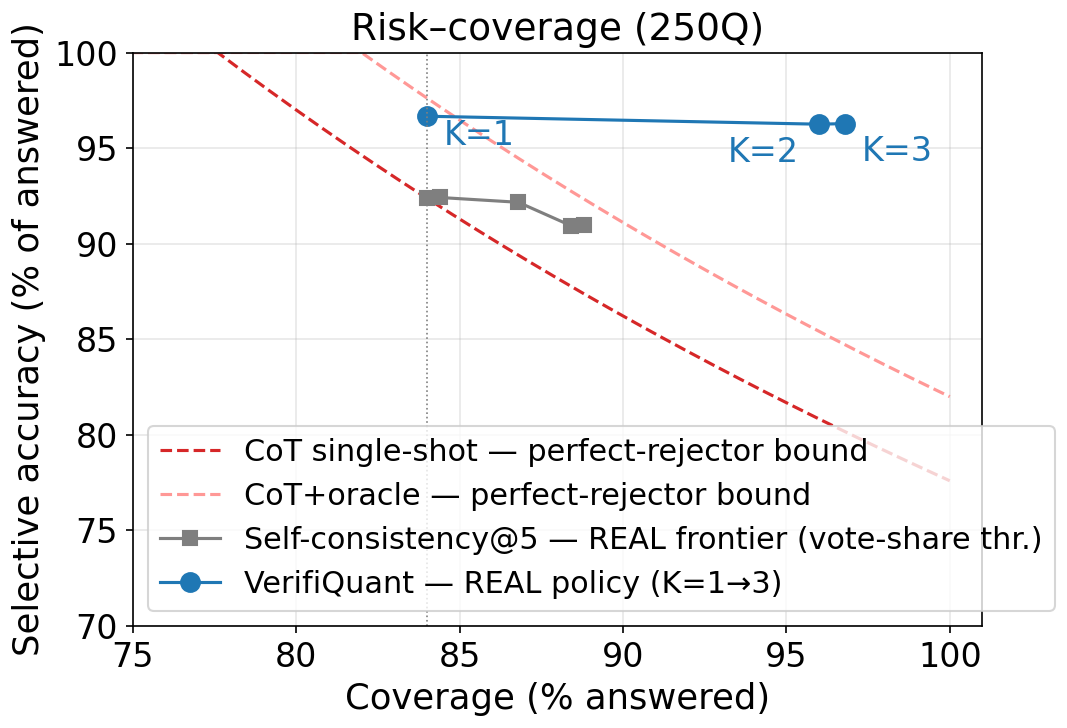
\includegraphics[width=0.9\linewidth]{figures/risk_coverage_250q.png}
\caption{Risk--coverage on 250Q.
Dashed curves: CoT baselines under a hypothetical \emph{perfect} rejector, which upper-bounds any real confidence threshold.
Gray squares: self-consistency@5, a \emph{realizable} confidence proxy using vote-share thresholds.
Blue: VerifiQuant's real operating points $K{=}1{\rightarrow}3$.
VerifiQuant's real autonomous point exceeds the single-shot perfect-rejector bound and the best realizable proxy alike.}
\label{fig:riskcov}
\end{figure}

\subsection{Residual-failure attribution and the audit loop}\label{sec:attribution}
Fifty-question pilots achieved SWR $=0\%$.
At 250 questions with a hard tier, silent wrongs appear, and we localize \emph{every} one.
Two attributions must not be conflated.
\emph{Runtime diagnostic attribution} names which gate and which check fired.
It is emitted at a structured exit with no gold answer.
\emph{Post-hoc research attribution} handles silent wrongs, which by definition escaped every gate.
It uses gold answers and the stored DiagnosticReport.
The taxonomy is not invented per error.
Before any run, the funnel leaves exactly three LLM-mediated steps fixed: contract \textbf{selection}, input \textbf{binding}, and declared-hint \textbf{recall}.
Each silent wrong is read off the trace: wrong \texttt{fic\_id}$\rightarrow$selection, wrong bound value$\rightarrow$binding, and undischarged declared hint$\rightarrow$recall.
The canonical run's \swResidualCanon{} silent wrongs all fall in these three classes.
\swCanonB{} are \emph{selection} failures, such as ``total interest'' routed to a ``lifetime cost'' card differing by exactly the principal.
\swCanonC{} are \emph{binding} failures, such as the annualization base 360 bound where a 90-day tenor was required.
\swCanonD{} are \emph{convention} failures.
In these cases, cards \emph{already declare} the exact ambiguity, yet the critic did not trigger it (declared 3/3, recalled 0/3; \S\ref{sec:recall}).
No residual falls outside these classes, and across all ${\sim}300$ evaluated questions no fourth kind appeared.
A separate build-time defect class was also found: three indicator cards returned a series instead of a scalar.
This was caught \emph{without gold answers} by a type audit and auto-repaired under the pre-declared output policy.
The post-audit canonical rerun is the run reported in Table~\ref{tab:main}.
The audit-repair loop explains why the reported run contains no surviving type-policy failures.

\emph{Canonical 50Q subset.} The original 50-question medium subset was used for protocol debugging and the full oracle/baseline grid.
The 250Q evaluation supersedes it as the primary evidence.
Two findings from that grid are load-bearing and we carry them forward.
First, even the strongest leak-free oracle configuration keeps SWR ${\geq}2\%$.
That is an architectural residue that deterministic execution removes.
Second, a JPMorgan multi-agent reimplementation answered all 50 questions at 14\% SWR without once triggering its own \texttt{ask\_human} node.
Possessing an escalation checkpoint is not the same as executing one.
These pilot findings are used only as supporting evidence; the 250Q evaluation remains the primary result.

%% ===== NOTE [CORE -- MAIN ADVANTAGE, keep] Trap resistance: malformed-input safety.
%% VQ 11.3% FNAR vs plain R-PAL 48.7% / prompted 27.5% (confirmatory 80-trap, CI [5.8,26.4]).
%% This is the real head-to-head win. Table 8 (tab:trap) is a headline table. =====
\subsection{Trap resistance}\label{sec:trap}
Traps have no legitimate numeric answer; correct behavior is interception (Table~\ref{tab:trap}).
All systems here are single-shot: VerifiQuant is evaluated funnel-only at $K{=}1$, and both R-PAL variants get one call.
With any oracle the ground-truth computation code re-injects redacted values and artificially defuses traps, so $K\geq2$ trap numbers would measure evaluation leakage, not capability.
The 80 traps are the balanced confirmatory set of \S\ref{sec:protocol}; each label \emph{is} its generating operator, and every E injection is verified to fire the contract's own predicate.

\begin{table}[t]
\caption{False numeric acceptance rate (FNAR) by operator on the balanced 80-trap confirmatory set (F/E/I/N, 20 each; 52 base questions, $\leq$2 operators each).
R-PAL is the retrieval-execution baseline; R-PAL$^{+}$ is the \emph{same} baseline handed the full M/N/F/E/I governance taxonomy in its prompt (mean of 3 runs).
Execution alone does not buy safety---plain R-PAL force-fits programs onto malformed questions (\govPlainFnar{} FNAR); prompting the taxonomy helps but does not reproduce executed gates.
M is not a valid trap and is excluded (see text).}
\label{tab:trap}
\small
\begin{tabular}{@{}lrrrl@{}}
\toprule
Operator (FNAR) & R-PAL & R-PAL$^{+}$ & VQ & VQ interception \\
\midrule
E (illegal boundary value) & 90\% & 30\% & \textbf{10\%} & \texttt{alert/E} \\
I (deleted disambiguator) & 95\% & 80\% & \textbf{20\%} & I\textsubscript{HARD/SOFT} \\
F (removed required input) & 10\% & 0\% & 10\% & \texttt{error/F} \\
N (out-of-scope ask) & 0\% & 0\% & 5\% & \texttt{refusal/N} \\
\midrule
Overall (F/E/I/N) & \govPlainFnar{} & \govPromptFnar{} & \textbf{\govVQfnar{}} & \\
\bottomrule
\end{tabular}
\end{table}

\emph{Executed gates, not prompted ones.}
The sharpest comparison is against R-PAL, which matched VerifiQuant on the clean set (Table~\ref{tab:main}).
On malformed inputs the same retrieval-execution machinery becomes a liability: plain R-PAL force-fits a program onto whatever it retrieves and reaches \govPlainFnar{} FNAR, concentrated on the E and I operators (90\% and 95\%).
Handing R-PAL the entire M/N/F/E/I governance taxonomy in its prompt (R-PAL$^{+}$) helps but does not close the gap: FNAR falls to \govPromptFnar{}, still \govGap{} points above VerifiQuant's \govVQfnar{}.
On a base-question-clustered bootstrap that keeps same-source perturbations and the three reruns grouped, the 95\% CI on this gap is $[\govCIlo{}, \govCIhi{}]$ points, excluding zero.
VerifiQuant also emits the \emph{right} structured exit more often: exact diagnostic \govVQdiag{} and exact action \govVQaction{}, versus \govPromptDiag{}/\govPromptAction{} for R-PAL$^{+}$.
Describing the gates in a prompt reproduces neither their interception rate nor their attribution.

The separation concentrates on E and I, the operators where correctness depends on a boundary or a convention rather than a present field.
Splitting the I stratum, VerifiQuant holds both halves (I\textsubscript{HARD} \govVQihard{}, I\textsubscript{SOFT} \govVQisoft{}) while R-PAL$^{+}$ degrades sharply (\govPromptIhard{}/\govPromptIsoft{}); the hard half is a small stratum ($n{=}6$; \S\ref{sec:limitations}) and we do not over-read it.
On F and N the systems are close: a missing required field and a blatant out-of-scope ask are conspicuous enough that prompting also intercepts them, and VerifiQuant's residual here (one N force-fit, two F) is a binding/selection slip, not a gate failure---but its exits still carry \texttt{diagnostic\_type}, \texttt{requested\_fields}, and routable actions that a prose refusal does not.
The M (under-specified intent) operator is excluded by construction: an under-specified question retains metric-bearing context, so the operator cannot isolate intent ambiguity from a resolvable metric, and no valid M-trap exists to score.
In the pilot every system---VerifiQuant included---emitted an unsafe number on the generator's M items, so open-ended intent ambiguity is a shared open problem, not a VerifiQuant-specific weakness.
The M-gate is exercised only qualitatively, on a genuinely metric-ambiguous prompt (``is this project worth investing in?'' with NPV, IRR, and payback all admissible), where the funnel abstains at \texttt{abstain/M} rather than silently picking one.
We make no quantitative trap claim for M; the quantitative boundary-declaration guarantee (C1) rests not on the conspicuous trap-N ask but on the retrieval near-OOD and out-of-library probes (\S\ref{sec:nearood},~\S\ref{sec:oodfam}), where an in-domain-looking question with its formula absent separates an executed scope gate from an unverified parametric guess.


%% ===== NOTE [CORE, keep] Governance Analysis: "governance does not transfer through
%% prompts" (executed vs prompted) + the OOD trade-off (6.1/6.2) + frontier (6.3) +
%% binding boundary (6.4). Full 12-cell multi-model refusal grid -> ACL; keep the conclusion. =====
\section{Governance Analysis}\label{sec:analysis}

\emph{Governance does not transfer through prompts.} Handing the same six-layer taxonomy to an oracle as prompt text does not reproduce structured refusal.
Neither variant emits a single diagnosable abstention.
It also \emph{degrades} blind-review accuracy: Flash falls to 92\% vs.\ 94\% plain, and Pro falls to 96\% vs.\ 98\%.
The guarantee lives in the executed gates, not their description.
Likewise, giving CoT an explicit refusal channel in a 12-cell prompt ablation makes it refuse non-selectively.
Refusals of would-have-been-correct answers outnumber rescued wrongs in every cell.
SWR falls only modestly, while accuracy collapses.
Prompted refusal lacks a gate's knowledge of \emph{which} check failed.
The reported oracle setting is the leak-free blind-review protocol; a deprecated GT-gated protocol was discarded because intervening only after wrong answers leaks the label.

%% ===== NOTE [TRADE-OFF / CORE-honesty, keep] OOD: NOT a win. libsweep = selective-
%% abstention is an architectural PROPERTY (tracks coverage). tab:oodsel = honest
%% 3-system trade-off (R-PAL more accurate OOD; VQ trades coverage for a scope signal;
%% no SWR win; VQ OOD selective acc 63.6% < R-PAL 95.5%). Verifiability-value -> future work/ACL. =====
\subsection{Abstention tracks library coverage}\label{sec:oodfam}
The coverage disclosure of \S\ref{sec:protocol} raises the question the main results cannot answer: what does the system do when the formula family is \emph{not} in the library?
We rebuild the library at nested fractions of the 250 families (10\%$\subset$25\%$\subset$50\%$\subset$75\%$\subset$100\%, pristine seeded builds) and rerun all 250 questions against each (Figure~\ref{fig:libsweep}).
VerifiQuant's abstention is \emph{selective}.
OOD abstention stays in a high band (91.6\%$\rightarrow$80.6\%), while ID abstention stays low (8.0\%$\rightarrow$14.4\%).
The 67--84-point separation holds at \emph{every} library size.
Abstention therefore tracks coverage as a property of the architecture, not of one operating point.
A refusal-permitted CoT baseline separates by only ${\sim}11$ points: its refusal is generic hedging, calibrated to nothing rather than to what the system can verify.
ID accuracy is flat (81.6--84.0\%, scale-normalized) as the library grows $10\times$.
The 100\%-coverage endpoint reproduces the canonical autonomous result (81.6\% vs.\ 81.2\% in Table~\ref{tab:kablation250}), giving an independent replication.
The one visible trade-off is honest.
OOD silent-wrong creeps from 1.3\% to 4.8\% as the library densifies.
Semantically adjacent cards make force-fitting more tempting.
This is the selection-frontier failure of \S\ref{sec:attribution}, now measured as a function of library density.

\begin{figure}[t]
\centering
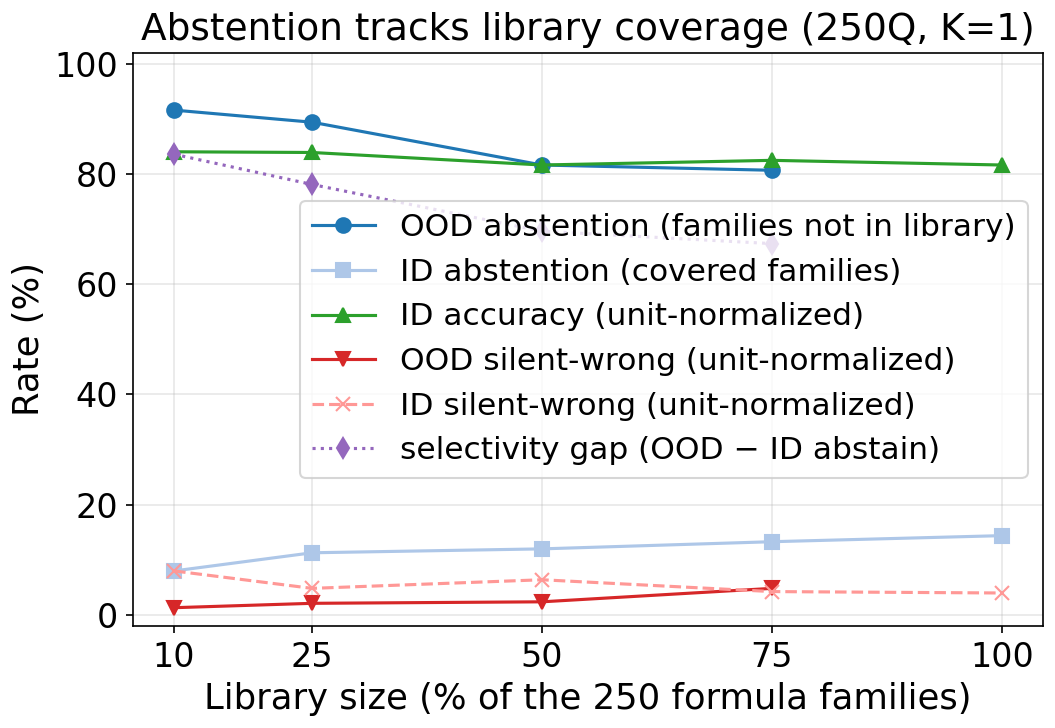
\includegraphics[width=0.9\linewidth]{figures/libsweep_250q.png}
\caption{Library-size sweep (250Q, $K{=}1$, nested pristine subset libraries).
Abstention tracks library coverage at every size.
OOD abstention (top band) vs.\ ID abstention (bottom band) keeps a 67--84-point gap.
ID accuracy is flat while the library grows $10\times$.
OOD silent-wrong rises only mildly with library density.}
\label{fig:libsweep}
\end{figure}

\emph{Selectivity, not raw abstention or accuracy, is the axis---and all three systems can be placed on it.}
On a fixed split (199 OOD, 51 ID; family present in the 50-family library or not) the systems occupy three regimes (Table~\ref{tab:oodsel}).
VerifiQuant abstains \oodVQabsOOD{} on OOD versus \oodVQabsID{} on ID---a \oodVQgap{}-point selectivity gap---so it answers few OOD questions but keeps each one contract-verified.
The retrieval-execution baseline is the opposite extreme: it abstains \oodRPALabsOOD{}, answering nearly every OOD question from parametric knowledge at \oodRPALcorrOOD{} correct---\emph{more} accurate out of library than VerifiQuant---but with \oodRPALswOOD{} silently wrong and no signal separating the two.
A refusal-permitted CoT sits between, abstaining \emph{indiscriminately} (\oodCoTabsOOD{} OOD vs \oodCoTabsID{} ID, an \oodCoTgap{}-point gap).
\emph{We state the trade-off plainly, since it runs against VerifiQuant.}
Governance does not make answers more correct out of library---it does not, and the cost is real: among the questions each system \emph{does} answer, VerifiQuant's out-of-library selective accuracy is only \oodVQselOOD{}, below CoT's \oodCoTselOOD{} and far below R-PAL's \oodRPALselOOD{}.
Its few non-abstentions are the selection-frontier slips of \S\ref{sec:attribution}, which is precisely why high abstention is the right default there.
A user who simply wants an answer to an out-of-library question is better served by R-PAL.
The only thing VerifiQuant provides here is the \emph{scope signal}---a structured, verified/unverified boundary that execution and prompting cannot emit---and its value is conditional on a deployment that requires provenance rather than a probable-but-untraceable number.
It does not reduce silent-wrong risk out of library, and whether that boundary is worth its coverage cost is a deployment question we leave to future work; the results here establish only that the boundary is \emph{selective} (it tracks coverage) and architectural (prompting does not reproduce it).

\begin{table}[t]
\caption{Out-of-library selectivity on a fixed split (199 OOD / 51 ID, family in the 50-family library or not).
The axis is scope awareness, not accuracy: R-PAL is the \emph{most} accurate on OOD yet almost never abstains; only VerifiQuant's abstention is selective (large OOD$-$ID gap).
$^{\dagger}$R-PAL ID abstention is taken from its clean-set coverage (it was not split-run on the 51 ID).}
\label{tab:oodsel}
\small
\begin{tabular}{@{}lrrrr@{}}
\toprule
System & OOD abstain & OOD correct & OOD SW & sel.\ gap (OOD$-$ID) \\
\midrule
CoT (refusal-permitted) & \oodCoTabsOOD{} & \oodCoTans{} & \oodCoTswOOD{} & \oodCoTgap{} \\
R-PAL & \oodRPALabsOOD{} & \oodRPALcorrOOD{} & \oodRPALswOOD{} & ${\approx}0^{\dagger}$ \\
\textbf{VerifiQuant} & \textbf{\oodVQabsOOD{}} & \oodVQcorrOOD{} & \oodVQswOOD{} & \textbf{\oodVQgap{}} \\
\bottomrule
\end{tabular}
\end{table}

%% ===== NOTE [TRADE-OFF | MERGE-candidate for 8pp] near-OOD: controlled per-question
%% companion to 6.1 (same trade-off message: scope signal, not accuracy). For 8pp this
%% can compress to 2-3 sentences folded into 6.1, or move to ACL. Not a standalone win. =====
\subsection{Retrieval near-OOD: scope awareness, not accuracy}\label{sec:nearood}
The library sweep removes families in bulk; a sharper question is what each system does when a \emph{single} question's target formula is absent but retrieval still returns something plausible.
We take \nearoodN{} in-library questions whose target family is the rank-1 hit and ablate that family under two conditions: \emph{bare} removes the target and its nearest neighbors; \emph{near-miss} removes only the target, leaving adjacent but inapplicable neighbors.
The ablation is applied identically to both systems at retrieval time.
\emph{The difference is scope awareness, not correctness.}
Plain R-PAL answers \emph{every} probe under both conditions (abstains 0\%): retrieval always returns some function, and with no scope gate the backbone writes a self-contained program and emits a number.
Those numbers are mostly \emph{right}---\nearoodRPALcorr{} match the gold answer, because the model knows the formula---but \nearoodRPALsw{} are silently wrong, and nothing marks which is which.
VerifiQuant instead abstains through the \texttt{N} scope gate on all \nearoodN{} bare probes (\nearoodVQbare{} answered) and all but two near-miss probes (\nearoodVQnear{} answered); the two exceptions are the selection-frontier slip of \S\ref{sec:attribution} (it bound to an adjacent neighbor), and near-miss being harder than bare is the predicted effect of leaving tempting neighbors in reach.
The claim is therefore \emph{not} that VerifiQuant is more accurate out of library---it is not, and it answers far fewer of these questions.
It is that VerifiQuant \emph{knows} the question is outside its verified library and R-PAL does not: R-PAL cannot separate a library-backed answer from a confident parametric guess, whereas VerifiQuant emits a number only when a contract applies.
This is the scope-boundary evidence the trap-N operator could not provide, where the out-of-scope ask was conspicuous enough for any system to refuse.
The probe is single-run over an in-library-derived set of \nearoodN{}, a mechanism result rather than a population estimate.

%% ===== NOTE [SUPPORT, compressible] hint-trigger frontier expansion (SWR ->1.2%).
%% Nice "mechanize a frontier" story but not load-bearing for the balance thesis;
%% compress or move detail to ACL if space is tight. =====
\subsection{The I-gate frontier is recall, not declaration}\label{sec:recall}
The class-D failures of \S\ref{sec:attribution} sharpen the standard ``LLM-dependent zone'' story with a measurement.
On all three convention failures, the contract had already declared the exact ambiguity.
One card's option text even reads ``\$3 per share''.
Yet the LLM critic triggered none of them (declared 3/3, recalled 0/3), silently adopting the default.
The contracts did their job; the binding constraint is \emph{declared-hint recall}.
This is mechanizable.
We prototype a deterministic trigger pre-pass.
If a convention-signal phrase (``per share'', ``as a percentage'', ``increased by'') appears verbatim in the question and the selected card declares a matching hint, the hint fires at its declared level without consulting the critic.
On the three recall failures the pre-pass fires all three at their declared levels while a clean-question control fires none.
We first validate it regression-free on the canonical 50Q set.
Accuracy remains 50/50, and the critic had independently recalled only 3 of 19 fired matches, an 84\% miss rate.
The pre-pass is then enabled on the full 250 questions.
It fires on 98 of 250 cases, with an 81\% critic recall-miss rate.
It converts all five medium-tier silent wrongs, including every class-D case, into correct, soft-flagged answers.
It cuts overall SWR from \vqSWRAll{} to \textbf{\vqtSWRAll{}}, with the medium tier at \textbf{\vqtSWRMed{}} (Table~\ref{tab:main}, last block).
The price is explicit and safe.
Four previously-correct cases now end in \emph{structured abstention}; these are hard triggers whose clarification did not converge.
They never become new silent wrongs.
The three remaining hard-tier failures are selection and binding cases outside any hint's reach.
Locating a frontier gap (\S\ref{sec:attribution}), mechanizing it, and buying an order-of-magnitude SWR reduction at a declared coverage cost is the frontier-expansion loop this architecture is designed around.
Moving hint recall from LLM judgment into the deterministic layer is exactly the frontier expansion the architecture is designed for; contract-declared machine-readable trigger keywords are the natural build-time extension.

%% ===== NOTE [ACL-candidate] input-binding / literal-grounding guard (Pro over-
%% normalization). Different axis (input provenance), prototype not evaluated online.
%% Strong 8pp cut candidate -> ACL; keep 1-2 sentences as a disclosed boundary if space allows. =====
\subsection{Where the guarantee ends: input binding}\label{sec:binding}
We disclose the sharpest boundary we know.
With a stronger underlying model (Pro), VerifiQuant produced silent wrongs sharing one pattern: \emph{over-normalization above the funnel}.
The model recomputed a literally-given input before binding.
In one case, a \$2.5M contract value silently became \$2.875M, adding profit the contract code would add again.
The result is positive, plausible, and passes every E-check: the funnel validates bound inputs and outputs, not whether a given value was rewritten during binding.
Notably the weaker model does not fail here (Flash binds the literal value): capability increases exploitation of whichever step is left unconstrained, so reliability tracks the constraint set, not model scale.
The direction is input-provenance checking: every bound value must trace to a literal context span.
We prototype a first version: a literal-grounding guard.
It admits a bound number only if it is derivable from a span in the question or context under a declared normalization.
Allowed normalizations include comma/currency stripping, percent$\leftrightarrow$decimal conversion, stated scale words, and time-basis conversion.
Otherwise, it downgrades a required field to \emph{missing} and routes it to the F gate as a structured request rather than a silent binding.
Replayed offline over the 250Q run, it flags 6.8\% of correct cases, which is the coverage it would cost.
It also catches the invented-value class, such as a \$50{,}000 ``invested amount'' present nowhere in the text.
The residual flags are \emph{derived-but-legal} bindings, such as a bond's coupon schedule built from face value and rate.
A full provenance schema would admit these cases by recording value, source span, normalization operation, and contract-declared derivation.
That schema is the natural next method contribution.

%% ===== NOTE [SUPPORT, compressible] Deployment: regulatory mapping (restates Table 1)
%% + cost numbers. Cost numbers are unique/keep; regulatory restatement already compressed. =====
\section{Deployment considerations}\label{sec:deployment}
We do not claim regulatory compliance, which involves organizational factors beyond any architecture; the six controls of Table~\ref{tab:spine} operationalize the recurring \emph{technical} demands of SR~11-7 \cite{fed2011sr117}, the EU AI Act \cite{euaiact2024} (Arts.~12--13), and FINRA \cite{finra2020ai}---failure-regime boundaries, input-to-output traceability, and explicit human checkpoints---as the M/N floor, the replayable DiagnosticReport five-tuple, and the I\textsubscript{HARD} hand-off.
Governance is also not the expensive part: VerifiQuant averages 1.20 funnel rounds and ${\approx}$3--4 LLM calls per case at 17.3\,s wall-clock, versus 6.3\,s for single-shot CoT and 27.8\,s for the CoT+oracle loop it outperforms, plus a one-time build cost of three LLM calls per formula family.

%% ===== NOTE [CORE, keep] Limitations: clean parity, OOD trade-off (no OOD win),
%% contract-derived trap set, I_HARD n=6, M unsolved, in-library scope. Honesty here is
%% load-bearing for the reviewer; keep dense but complete. =====
\section{Limitations}\label{sec:limitations}
VerifiQuant reduces and localizes silent wrongs; it does not eliminate them, and residual attribution uses gold answers unavailable in deployment.
On clean, well-posed questions a retrieval-grounded execution baseline (R-PAL) matches VerifiQuant on accuracy and silent-wrong rate; our advantage is on malformed inputs, not clean-set scalar accuracy.
\emph{Out of library the trade-off runs against us:} R-PAL answers more out-of-library questions correctly (\oodRPALcorrOOD{}) than VerifiQuant, VerifiQuant's own out-of-library selective accuracy is only \oodVQselOOD{}, and its abstention does \emph{not} lower silent-wrong risk there; the sole benefit is a scope signal whose value depends on a deployment that requires provenance, and quantifying when that boundary is worth its coverage cost is future work.
The governance advantage is measured on an 80-trap balanced confirmatory set derived from VerifiQuant's own contracts, which is mechanism-aligned and may favor a contract-gated system; each E injection is verified against the contract predicate, but the I\textsubscript{HARD} stratum is small ($n{=}6$, the phrase-deletion ceiling) and an independently authored messy-query set remains the natural external-validity test.
Our evaluation covers single-question, formula-grounded numerical QA, not full workflow governance over documents, tables, conflicting sources, or jurisdictional policy.
The guarantees are conditional on faithful input binding, contract quality, an intent-explicit oracle, and one formula-provenance benchmark/backbone family.
The M gate is demonstrated qualitatively but not quantified---and no system in our study handles open-ended intent ambiguity---while the literal-grounding guard is still prototype-grade.
Soft-warning lifecycle is also unresolved: a warning should only be cleared when the dimension it names has been resolved, since one Pro case cleared a warning while the error persisted.
Broader benchmarks, realistic human studies, and cross-vendor replication remain future work.

%% ===== NOTE [CORE, keep] Conclusion: balance = clean parity + malformed-input safety;
%% OOD stated as deliberate trade-off (no OOD win). Keep tight. =====
\section{Conclusion}
Financial LLM deployment is blocked less by what models get wrong than by what systems cannot govern.
Six governance controls demanded by regulators can be compiled into the reasoning pipeline as executable mechanisms.
These controls are boundary declaration, input validation, ambiguity disclosure, cross-verified repair, audit-replayable traces, and selective abstention.
At 250 questions across two difficulty tiers, a retrieval-grounded execution baseline matches the system on clean, well-posed questions, and it dominates prompt-governed CoT baselines on accuracy and silent-wrong rate.
The system earns its keep on \emph{malformed} inputs---missing fields, boundary violations, unresolved conventions---where a confident number is by construction wrong and executed gates intercept what execution and prompting force-fit.
Out of library it makes a deliberate trade: it abstains selectively, buying a verified/unverified boundary at a coverage cost rather than a more accurate answer, and we are explicit that this does not lower silent-wrong risk there.
It also post-hoc localizes every residual failure to one of three pre-declared frontier classes, and repairs its own contract defects under pre-declared policy with a full audit trail.
None of this transfers through prompts: describing the funnel degrades a blind oracle, and prompted refusal misfires.
A governed system will sometimes say less.
Everything it says is attributable and audit-replayable.
Where it cannot verify, it refuses honestly.
In high-stakes finance, an auditable refusal is worth more than an unauditable answer.
